\documentclass[10pt,twocolumn,letterpaper]{article}
\usepackage[letterpaper,top=1.8cm,bottom=2.0cm,left=1.7cm,right=1.7cm,columnsep=0.7cm]{geometry}
\usepackage[T1]{fontenc}
\usepackage{mathptmx}
\usepackage{microtype}
\usepackage{booktabs}
\usepackage{graphicx}
\usepackage{amsmath,amssymb}
\usepackage{array}
\usepackage[hidelinks,colorlinks=false]{hyperref}
\hypersetup{pdftitle={Is the Confidence Trustworthy? A Hard Synthetic Benchmark for Power-Equipment Inspection Labels}, pdfauthor={fe2131-art}, pdfsubject={Synthetic benchmark, calibration and selective prediction}}
\usepackage{pgfplots}
\pgfplotsset{compat=1.18, every axis/.append style={font=\footnotesize, tick label style={font=\scriptsize}, label style={font=\footnotesize}, legend style={font=\scriptsize, draw=none, fill=none}}}
\usepgfplotslibrary{groupplots}
\raggedbottom
\setlength{\textfloatsep}{8pt plus 2pt minus 2pt}
\setlength{\floatsep}{6pt plus 2pt minus 2pt}
\setlength{\intextsep}{6pt plus 2pt minus 2pt}
\setlength{\abovecaptionskip}{3pt}
\setlength{\belowcaptionskip}{0pt}
\renewcommand{\arraystretch}{1.08}
\setlength{\parskip}{0pt}
\setlength{\parindent}{1.0em}
\makeatletter
\renewcommand\section{\@startsection{section}{1}{\z@}{8pt plus 2pt minus 1pt}{4pt}{\normalfont\small\bfseries\MakeUppercase}}
\renewcommand\subsection{\@startsection{subsection}{2}{\z@}{6pt plus 2pt minus 1pt}{2pt}{\normalfont\small\bfseries\itshape}}
\makeatother
\renewcommand{\refname}{References}

\title{\LARGE\bfseries Is the Confidence Trustworthy? \\[2pt] A Hard Synthetic Benchmark for Power-Equipment Inspection Labels}
\author{\normalsize fe2131-art\\[-2pt]{\small\texttt{github.com/fe2131-art/power-decision-benchmark}}}
\date{\small November 2026}

\begin{document}
\twocolumn[{%
\begin{center}
{\LARGE\bfseries Is the Confidence Trustworthy?}\\[3pt]
{\Large\bfseries A Hard Synthetic Benchmark for Power-Equipment Inspection Labels}\\[8pt]
{\normalsize fe2131-art}\\[1pt]
{\small Code, data, and result tables: \url{https://github.com/fe2131-art/power-decision-benchmark}}\\[10pt]
\end{center}
\begin{minipage}{0.92\textwidth}
\small\textbf{Abstract---}Maintenance records of power equipment are free text, and automated labelling helps only if the reported confidence can decide which outputs to accept. We build a hard synthetic benchmark of 474 inspection records with three structured fields (equipment, observed event, cause status). The records are split by scenario family into 124 calibration and 350 held-out test cases. We evaluate nine systems: two GPT-6 Luna interfaces, Qwen3.8-27B, two sizes of the kev decision model in two precisions, Clef-Flash, and d1-2B. Probabilities come from native decision outputs or from output-token log-probabilities. We report exact-match accuracy with family-level bootstrap intervals, per-field calibration, and selective prediction whose threshold is chosen only on calibration data. On the held-out set, Clef-Flash has the highest exact-match accuracy (0.954), but its equipment probabilities are poorly calibrated (ECE 0.159). The intervals of the top systems overlap. Calibration varies by field and system, and log-probability estimates saturate on clear cases. The records are synthetic and labelled by the authors, so the results describe the benchmark, not field performance.\par
\vspace{4pt}
\small\textbf{Index Terms---}LLM evaluation, decision models, calibration, selective prediction, power equipment, synthetic benchmark.
\end{minipage}
\vspace{10pt}
}]

\section{Introduction}
Inspection records for power equipment are written in free text by field staff, and they are often incomplete or contradictory. Automated labelling can support analysis and triage, but a label is only useful downstream if two things are known: how often it is exactly right, and whether the confidence attached to it can decide which outputs may be accepted without review. Generative language models give fluent labels but do not expose calibrated probabilities. Purpose-built decision models expose a distribution over options, but their calibration is rarely measured on hard cases.

We study both questions on one benchmark. Our contributions are: (i) a 474-record synthetic benchmark whose hard cases include corrections, retractions, negations, resolved events, cross-device confusion, and cause-contrast triplets, split by scenario family; (ii) a comparison of nine systems covering generative models, an API decision model, and four local decision models, with probabilities obtained in a uniform way; and (iii) an audit that reports exact-match accuracy with cluster-level intervals, per-field calibration, and selective prediction with a threshold fixed on calibration data before the test set is seen.

\section{Benchmark}
The benchmark contains 474 synthetic inspection records written by the authors. Of these, 408 are generated from equipment-by-event templates, 24 describe normal states, and 42 are hand-written boundary cases. They fall into 47 scenario families. Each record has three labels: \emph{equipment} (six options), \emph{observation} (eight options), and \emph{cause status} (confirmed, suspected, or unknown). The labels were assigned by design, not by field engineers, so they stand in for expert judgement and are not a field gold standard.

The records are split into a calibration set (124 records, used only to choose a threshold) and a held-out test set (350 records). The split is by family, so near-duplicate records never appear on both sides. The split manifest records the seed, case and family IDs, and SHA-256 hashes of every file. The test set contains 104 cause-contrast triplets: three records that differ only in cause status.

\section{Systems and Probability Sources}
Table~\ref{tab:systems} summarises the systems. Native decision models return a distribution over options directly: the Decisions API, Clef-Flash, d1-2B, and kev. For the two generative systems (GPT-6 Luna through the Responses API, and Qwen3.8-27B), we request output-token log-probabilities and renormalise the probabilities of the candidate values at the first token of each field. Multi-token values are therefore approximated by their first token. Self-reported probabilities are not used, because they are not a property of the model's output distribution.

\begin{table}[t]
\centering
\caption{Systems compared. ``logprob'' denotes a first-token log-probability approximation.}
\label{tab:systems}
\small
\begin{tabular}{@{}lll@{}}
\toprule
System & Probabilities & Runtime \\
\midrule
GPT-6 Luna, Responses & logprob & OpenAI API \\
GPT-6 Luna, Decisions API & native & OpenAI API \\
Qwen3.8-27B, UD-Q4\_K\_M & logprob & llama.cpp, V100 \\
kev 9B / 0.8B, Q8\_0 and BF16 & native & Ollama, V100 \\
Clef-Flash, Q8\_0 & native & llama.cpp, V100 \\
d1-2B, Q8\_0 & native & llama.cpp, V100 \\
\bottomrule
\end{tabular}
\end{table}

\section{Evaluation Protocol}
\textbf{Accuracy.} A record is correct only if all three fields are correct. Accuracy is computed over all planned cases, so failed requests count as errors. Intervals are 95\% cluster bootstrap intervals over scenario families (1000 resamples), because records from one family are not independent.

\textbf{Calibration.} For each field we compute the expected calibration error with 10 equal-width bins (ECE) and the multiclass Brier score~\cite{brier1950}. ECE follows the binned formulation of~\cite{naeini2015,guo2017}.

\textbf{Selective prediction.} A record is accepted when its lowest selected-option probability reaches a threshold~\cite{geifman2017}. The threshold is the lowest value on the calibration set at which the observed error rate is at most 5\% and at least 10 records are accepted. It is then applied unchanged to the test set. The 5\% budget is an evaluation condition chosen for comparison; it is not a safety guarantee.

\textbf{Triplets.} A triplet counts as correct only when all three of its records are labelled correctly.

\section{Results}
Table~\ref{tab:acc} and Fig.~\ref{fig:acc} report exact-match accuracy on the test set. The intervals of the top systems overlap, so we do not rank them. Clef-Flash has the highest point estimate; Table~\ref{tab:acc} gives the numbers behind Fig.~\ref{fig:acc}.

\begin{table}[t]
\centering
\caption{Exact-match accuracy on the 350 test records with 95\% cluster bootstrap intervals, and per-case latency (one run per system, ms).}
\label{tab:acc}
\small
\setlength{\tabcolsep}{3.5pt}
\begin{tabular}{@{}lcccc@{}}
\toprule
System & Exact & 95\% CI & p50 & p95 \\
\midrule
GPT-6 Luna (logprob) & 0.940 & [0.861, 0.991] & 1,309 & 6,642 \\
GPT-6 Luna (Decisions) & 0.920 & [0.832, 0.986] & 301 & 401 \\
Qwen3.8-27B (logprob) & 0.931 & [0.851, 0.984] & 1,998 & 2,223 \\
kev 9B (Q8\_0) & 0.880 & [0.800, 0.941] & 503 & 510 \\
kev 9B (BF16) & 0.877 & [0.797, 0.937] & 1,263 & 1,297 \\
kev 0.8B (Q8\_0) & 0.554 & [0.450, 0.649] & 139 & 146 \\
kev 0.8B (BF16) & 0.549 & [0.447, 0.641] & 221 & 230 \\
Clef-Flash (Q8\_0) & 0.954 & [0.912, 0.986] & 286 & 288 \\
d1-2B (Q8\_0) & 0.877 & [0.791, 0.948] & 116 & 120 \\
\bottomrule
\end{tabular}
\end{table}

\begin{figure*}[t]
\centering
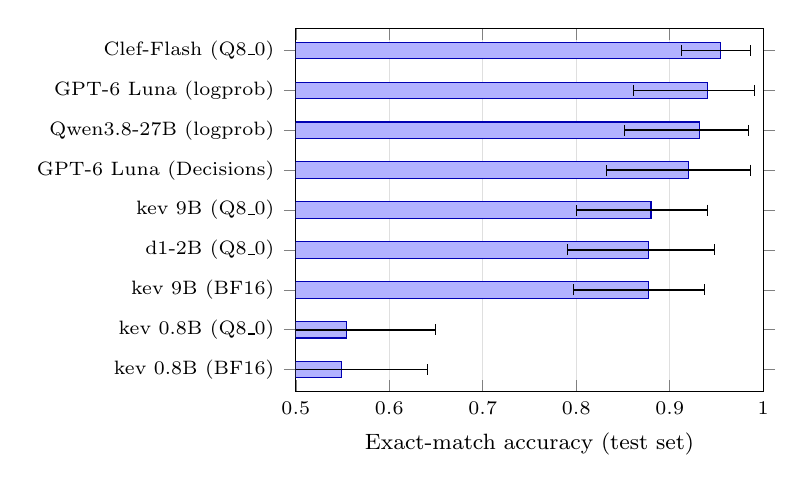
\begin{tikzpicture}
\begin{axis}[
  xbar, width=0.62\textwidth, height=6.2cm, bar width=6pt,
  xmin=0.5, xmax=1.0, xtick={0.5,0.6,0.7,0.8,0.9,1.0},
  xlabel={Exact-match accuracy (test set)},
  ytick={0,1,2,3,4,5,6,7,8}, yticklabels={{kev 0.8B (BF16)},{kev 0.8B (Q8\_0)},{kev 9B (BF16)},{d1-2B (Q8\_0)},{kev 9B (Q8\_0)},{GPT-6 Luna (Decisions)},{Qwen3.8-27B (logprob)},{GPT-6 Luna (logprob)},{Clef-Flash (Q8\_0)}},
  enlarge y limits=0.07, xmajorgrids=true, grid style={gray!25},
]
\addplot+[fill=blue!30, draw=blue!70!black, error bars/.cd, x dir=both, x explicit, error bar style={line width=0.6pt, black}]
coordinates {(0.5486,0) += (0.0923,0) -= (0.1013,0) %
  (0.5543,1) += (0.0948,0) -= (0.1043,0) %
  (0.8771,2) += (0.0600,0) -= (0.0797,0) %
  (0.8771,3) += (0.0707,0) -= (0.0865,0) %
  (0.8800,4) += (0.0609,0) -= (0.0800,0) %
  (0.9200,5) += (0.0660,0) -= (0.0876,0) %
  (0.9314,6) += (0.0527,0) -= (0.0800,0) %
  (0.9400,7) += (0.0510,0) -= (0.0792,0) %
  (0.9543,8) += (0.0319,0) -= (0.0419,0)};
\end{axis}
\end{tikzpicture}
\caption{Exact-match accuracy on the test set. Bars are point estimates; whiskers are 95\% cluster bootstrap intervals.}
\label{fig:acc}
\end{figure*}

Fig.~\ref{fig:cal} shows reliability for the equipment field (left) and the risk–coverage trade-off as the selection threshold varies (right). Table~\ref{tab:cal} gives the numerical calibration and selective-prediction results at the 5\% budget.

\begin{figure*}[t]
\centering
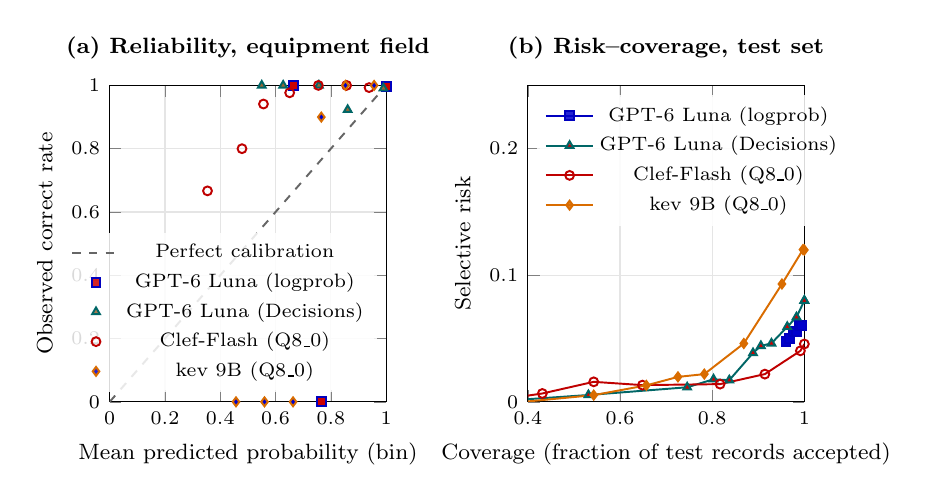
\begin{tikzpicture}
\begin{groupplot}[
  group style={group size=2 by 1, horizontal sep=1.8cm},
  width=0.42\textwidth, height=5.6cm, grid=major, grid style={gray!20},
  every axis plot/.append style={line width=0.7pt},
  legend style={font=\scriptsize, draw=none, fill=white, fill opacity=0.85, text opacity=1}
]
\nextgroupplot[
  xmin=0, xmax=1, ymin=0, ymax=1,
  xlabel={Mean predicted probability (bin)}, ylabel={Observed correct rate},
  xtick={0,0.2,0.4,0.6,0.8,1}, ytick={0,0.2,0.4,0.6,0.8,1},
  legend pos=south east, title={(a) Reliability, equipment field}, title style={font=\footnotesize\bfseries}
]
\addplot[black!60, dashed, no markers, domain=0:1] {x};
\addlegendentry{Perfect calibration}
\addplot+[blue!75!black, mark=square*, mark size=1.6pt, only marks, line width=0.7pt] coordinates {(0.6641,1.0000) (0.7664,0.0000) (1.0000,0.9971)};
\addlegendentry{GPT-6 Luna (logprob)}
\addplot+[teal!80!black, mark=triangle*, mark size=1.6pt, only marks, line width=0.7pt] coordinates {(0.5500,1.0000) (0.6275,1.0000) (0.7567,1.0000) (0.8608,0.9231) (0.9902,0.9909)};
\addlegendentry{GPT-6 Luna (Decisions)}
\addplot+[red!75!black, mark=o, mark size=1.6pt, only marks, line width=0.7pt] coordinates {(0.3538,0.6667) (0.4786,0.8000) (0.5562,0.9412) (0.6510,0.9767) (0.7548,1.0000) (0.8569,1.0000) (0.9382,0.9931)};
\addlegendentry{Clef-Flash (Q8\_0)}
\addplot+[orange!85!black, mark=diamond*, mark size=1.6pt, only marks, line width=0.7pt] coordinates {(0.4569,0.0000) (0.5600,0.0000) (0.6633,0.0000) (0.7655,0.9000) (0.8529,1.0000) (0.9565,1.0000)};
\addlegendentry{kev 9B (Q8\_0)}
\nextgroupplot[
  xmin=0.4, xmax=1.0, ymin=0, ymax=0.25,
  xlabel={Coverage (fraction of test records accepted)}, ylabel={Selective risk},
  legend pos=north west, title={(b) Risk--coverage, test set}, title style={font=\footnotesize\bfseries}
]
\addplot+[blue!75!black, mark=square*, mark size=1.6pt, thick, line width=0.7pt] coordinates {(0.9600,0.0476) (0.9600,0.0476) (0.9600,0.0476) (0.9600,0.0476) (0.9600,0.0476) (0.9686,0.0501) (0.9771,0.0556) (0.9771,0.0556) (0.9771,0.0556) (0.9829,0.0552) (0.9886,0.0607) (0.9914,0.0605) (0.9943,0.0603) (0.9943,0.0603) (0.9943,0.0603)};
\addlegendentry{GPT-6 Luna (logprob)}
\addplot+[teal!80!black, mark=triangle*, mark size=1.6pt, thick, line width=0.7pt] coordinates {(0.0114,0.0000) (0.0114,0.0000) (0.0114,0.0000) (0.3171,0.0000) (0.5314,0.0054) (0.7457,0.0115) (0.8029,0.0178) (0.8371,0.0171) (0.8886,0.0386) (0.9057,0.0442) (0.9286,0.0462) (0.9629,0.0593) (0.9829,0.0669) (1.0000,0.0800) (1.0000,0.0800)};
\addlegendentry{GPT-6 Luna (Decisions)}
\addplot+[red!75!black, mark=o, mark size=1.6pt, thick, line width=0.7pt] coordinates {(0.0171,0.0000) (0.1771,0.0000) (0.3086,0.0000) (0.4314,0.0066) (0.5429,0.0158) (0.6486,0.0132) (0.8171,0.0140) (0.9143,0.0219) (0.9914,0.0403) (1.0000,0.0457)};
\addlegendentry{Clef-Flash (Q8\_0)}
\addplot+[orange!85!black, mark=diamond*, mark size=1.6pt, thick, line width=0.7pt] coordinates {(0.1686,0.0000) (0.3914,0.0000) (0.5429,0.0053) (0.6571,0.0130) (0.7257,0.0197) (0.7829,0.0219) (0.8686,0.0461) (0.9514,0.0931) (0.9971,0.1203) (1.0000,0.1200)};
\addlegendentry{kev 9B (Q8\_0)}
\end{groupplot}
\end{tikzpicture}
\caption{Calibration and selective prediction on the test set for four systems. (a)~Reliability diagram for the equipment field (10 equal-width bins; markers are bin means; the dashed diagonal is perfect calibration). (b)~Risk--coverage curves; each point is a selection threshold, and a lower curve is better at the same coverage.}
\label{fig:cal}
\end{figure*}

\begin{table*}[t]
\centering
\caption{Calibration and selective prediction on the test set. ECE uses 10 bins; Brier is for the observation field. Coverage and risk use the threshold chosen on calibration data for a 5\% budget. Triplet is the cause-contrast accuracy.}
\label{tab:cal}
\small
\setlength{\tabcolsep}{3pt}
\begin{tabular}{@{}lcccccccc@{}}
\toprule
System & \multicolumn{3}{c}{ECE} & Brier & \multicolumn{2}{c}{Selective} & \multicolumn{1}{c}{Triplet} \\
\cmidrule(lr){2-4}\cmidrule(lr){6-7}
 & equip. & obs. & cause & obs. & coverage & risk & acc. \\
\midrule
GPT-6 Luna (logprob) & 0.006 & 0.045 & 0.008 & 0.093 & 0.977 & 0.056 & 0.990 \\
GPT-6 Luna (Decisions) & 0.011 & 0.031 & 0.006 & 0.089 & 1.000 & 0.080 & 1.000 \\
Qwen3.8-27B (logprob) & 0.011 & 0.023 & 0.004 & 0.335 & 0.806 & 0.071 & 1.000 \\
kev 9B (Q8\_0) & 0.073 & 0.062 & 0.066 & 0.098 & 0.997 & 0.120 & 0.942 \\
kev 9B (BF16) & 0.072 & 0.059 & 0.064 & 0.101 & 0.997 & 0.120 & 0.923 \\
kev 0.8B (Q8\_0) & 0.318 & 0.356 & 0.319 & 0.536 & 0.069 & 0.083 & 0.683 \\
kev 0.8B (BF16) & 0.317 & 0.348 & 0.319 & 0.539 & 0.094 & 0.061 & 0.683 \\
Clef-Flash (Q8\_0) & 0.159 & 0.137 & 0.054 & 0.073 & 0.991 & 0.040 & 1.000 \\
d1-2B (Q8\_0) & 0.072 & 0.093 & 0.059 & 0.143 & 0.863 & 0.046 & 0.981 \\
\bottomrule
\end{tabular}
\end{table*}

The latency columns of Table~\ref{tab:acc} give the p50 and p95 time per case. Each system ran alone, one after another, so the times are comparable within a deployment but not across deployments: OpenAI timings include network latency, and the local systems ran on one V100 32\,GB with different serving stacks.



\section{Discussion and Limitations}
\textbf{Accuracy.} The top systems have overlapping intervals, so the ranking is not established. The highest point estimate, Clef-Flash (0.954), also has the worst equipment calibration among the top systems (ECE 0.159). Its selective policy accepts 99\% of records at a 4.0\% error rate on the accepted set, so the threshold does not filter out its errors.

\textbf{Calibration.} Calibration depends on the field. GPT-6 Luna (logprob) has the lowest equipment ECE (0.006), and Qwen3.8-27B has the lowest observation ECE of all nine systems (0.023). Log-probability estimates saturate for clear cases, so their small ECE values partly reflect probabilities close to 1; they should not be read as proof of calibration. The smallest kev model is far less accurate than the rest (0.554), and its probabilities are poorly calibrated (ECE about 0.32).

\textbf{Precision.} The BF16 and Q8\_0 versions of kev give nearly the same accuracy and calibration. BF16 is slower (1,263 ms against 503 ms at p50 for 9B) on this hardware.

\textbf{Limitations.} The data are synthetic and were written by the same people who designed the metrics. There is no expert-reviewed gold standard. Each system was run once. Intervals are cluster-level and wide. Qwen was run at temperature 0, while the other systems used service defaults. The 5\% budget is a chosen condition, not a guarantee. The results support comparisons on this benchmark; they do not establish field performance.

\section{Conclusion}
On a hard synthetic benchmark of power-equipment inspection records, the systems that score highest on exact-match accuracy are not the ones with the most reliable probabilities. Accuracy, calibration, and selective prediction should be reported separately, with intervals that account for dependence between related records. The benchmark, the split manifests, and the audit scripts are published so that these comparisons can be repeated.

\begin{thebibliography}{99}
\bibitem{brier1950} G.~W.~Brier, ``Verification of forecasts expressed in terms of probability,'' \emph{Monthly Weather Review}, vol.~78, no.~1, pp.~1--3, 1950.
\bibitem{naeini2015} M.~P.~Naeini, G.~F.~Cooper, and M.~Hauskrecht, ``Obtaining well calibrated probabilities using Bayesian binning,'' in \emph{Proc. AAAI}, 2015.
\bibitem{guo2017} C.~Guo, G.~Pleiss, Y.~Sun, and K.~Q.~Weinberger, ``On calibration of modern neural networks,'' in \emph{Proc. ICML}, 2017.
\bibitem{geifman2017} Y.~Geifman and R.~El-Yaniv, ``Selective classification for deep neural networks,'' in \emph{Advances in NeurIPS}, 2017.
\end{thebibliography}

\end{document}
